With various architectures and organizations, servers deployed at
different supercomputers have different characteristics in terms of
power consumption. The static power ratio $\rho$ is used to abstract the
amount of static power consumed versus dynamic power. In our models,
$\rho$ does not impact the completion time, but power and energy consumption.
Considering modern systems, we vary $\rho$ from 0.3 to 0.7 and study its effect
on the expected energy consumption. The results for Lazy Shadowing with $\alpha=5$ are normalized to that of process replication and shown in 
Figure~\ref{fig:power_ratio}. The results for other values of $\alpha$ have similar behavior and thus are not shown. Lazy Shadowing achieves
more energy saving when static power ratio is low, since it saves dynamic 
power but not static power. When static power ratio is low ($\rho=0.3$), Lazy Shadowing
is able to save 20\%-24\% energy for the MTBF of 5 to 25 years. The saving decreases to 5\%-11\% when $\rho$ reaches 0.7. 

\begin{figure}[!t]
	\begin{center}
		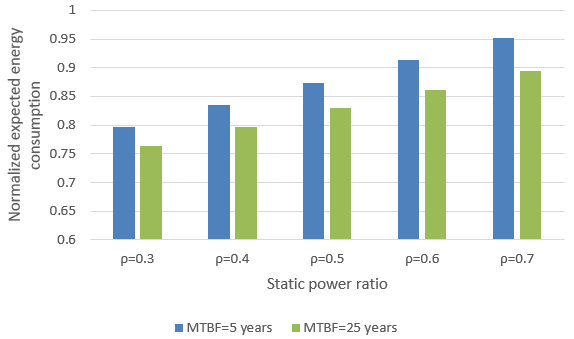
\includegraphics[width=\columnwidth]{Figures/s_power_5}
	\end{center}
	%\vskip -0.22in 
	\caption{Impact of static power ratio on energy consumption normalized to process replication. $W=10^6$ hours, $N=10^6$, $\alpha$=5.}
	\label{fig:power_ratio}
\end{figure}